

\documentclass[12pt]{article}
\usepackage{graphicx}
\usepackage{amsmath}
\usepackage{listings}
\usepackage{color}
\usepackage[section]{placeins} %this stops the figures from showing up in wrong section

\definecolor{dkgreen}{rgb}{0,0.6,0}
\definecolor{dkblue}{rgb}{0,0.0,0.6}
\definecolor{dkred}{rgb}{0.9,0.0,0.1}


\begin{document}

\lstset{language=Fortran,tabsize=4,numbers=left,numberstyle=\tiny,basicstyle=\ttfamily\small\color{dkblue},stringstyle=\ttfamily\color{blue},keywordstyle=\rmfamily\color{dkred}\bfseries\emph,backgroundcolor=\color{white},commentstyle=\color{dkgreen}}




\title{Physics 562 - Computational Physics\\[.5cm]
Assignment 2: Quantum Harmonic Oscillator}
\author{Josh Fernandes\\
Department of Physics \& Astronomy\\
California State University Long Beach}
\date{\today}

  
\maketitle



\begin{abstract}
The assignment focuses on solving for the eigenfunctions for the one dimensional quantum harmonic oscillator. In the process, programs to imitate the exponential function, hermit function, and factorial function are created. The ground state and the first six excited states are plotted on a graph. The results are not normalized, so this paper only concludes that the amplitude decreases and the wavelength decreases as the energy state is increased.
\end{abstract}

\section{Introduction}\label{s:intro}

While the classical harmonic oscillator is well suited for solving systems of mechanical springs and pendulums, the quantum harmonic oscillator can solves systems of atomic particles. In addition, the quantum harmonic oscillator is one of the few quantum mechanical systems that has an exact, analytical solution. The eigenfunctions for the quantum harmonic oscillator are of the form

\begin{gather}
\Psi_n(x) = \frac{1}{\sqrt{2^n \, n!}}\cdot \left(\frac{mw}{\pi \hbar}\right)^{\frac{1}{4}} \cdot e^{-\frac{mwx^2}{2\hbar}} \cdot H_n \left(\sqrt{\frac{mw}{\hbar}} \, x \right).
\end{gather}

The parameters are set as $m=1$, $w=1$, and $\hbar=3$. Although these values have no physical meaning, they preserve the shape of the curves. The first seven energy states are plotted in order to determine traits about the curves.
\section{The Fortran95 code}

The code is going to solve the problem. First a module called {\tt NumType} is created to store all my global parameters. These include values of pi and the exponential of one. 


The main program is {\tt oscillator} and it begins with its own module. In this module, I call in numtype.



The code is run by typing {\tt ./wowza}. The results are printed on the screen, or the data can redirect to the file {\tt amazing data} by typing {\tt ./wowza > amazingdata.data}. The {\tt Plot} provides the picture in Fig.\ \ref{orbitstuff}. 

\section{Data Analysis}

the code returns an array of values.

\begin {figure}[!htb]
	\resizebox{\columnwidth}{!}{% GNUPLOT: LaTeX picture with Postscript
\begingroup
  \makeatletter
  \providecommand\color[2][]{%
    \GenericError{(gnuplot) \space\space\space\@spaces}{%
      Package color not loaded in conjunction with
      terminal option `colourtext'%
    }{See the gnuplot documentation for explanation.%
    }{Either use 'blacktext' in gnuplot or load the package
      color.sty in LaTeX.}%
    \renewcommand\color[2][]{}%
  }%
  \providecommand\includegraphics[2][]{%
    \GenericError{(gnuplot) \space\space\space\@spaces}{%
      Package graphicx or graphics not loaded%
    }{See the gnuplot documentation for explanation.%
    }{The gnuplot epslatex terminal needs graphicx.sty or graphics.sty.}%
    \renewcommand\includegraphics[2][]{}%
  }%
  \providecommand\rotatebox[2]{#2}%
  \@ifundefined{ifGPcolor}{%
    \newif\ifGPcolor
    \GPcolortrue
  }{}%
  \@ifundefined{ifGPblacktext}{%
    \newif\ifGPblacktext
    \GPblacktexttrue
  }{}%
  % define a \g@addto@macro without @ in the name:
  \let\gplgaddtomacro\g@addto@macro
  % define empty templates for all commands taking text:
  \gdef\gplbacktext{}%
  \gdef\gplfronttext{}%
  \makeatother
  \ifGPblacktext
    % no textcolor at all
    \def\colorrgb#1{}%
    \def\colorgray#1{}%
  \else
    % gray or color?
    \ifGPcolor
      \def\colorrgb#1{\color[rgb]{#1}}%
      \def\colorgray#1{\color[gray]{#1}}%
      \expandafter\def\csname LTw\endcsname{\color{white}}%
      \expandafter\def\csname LTb\endcsname{\color{black}}%
      \expandafter\def\csname LTa\endcsname{\color{black}}%
      \expandafter\def\csname LT0\endcsname{\color[rgb]{1,0,0}}%
      \expandafter\def\csname LT1\endcsname{\color[rgb]{0,1,0}}%
      \expandafter\def\csname LT2\endcsname{\color[rgb]{0,0,1}}%
      \expandafter\def\csname LT3\endcsname{\color[rgb]{1,0,1}}%
      \expandafter\def\csname LT4\endcsname{\color[rgb]{0,1,1}}%
      \expandafter\def\csname LT5\endcsname{\color[rgb]{1,1,0}}%
      \expandafter\def\csname LT6\endcsname{\color[rgb]{0,0,0}}%
      \expandafter\def\csname LT7\endcsname{\color[rgb]{1,0.3,0}}%
      \expandafter\def\csname LT8\endcsname{\color[rgb]{0.5,0.5,0.5}}%
    \else
      % gray
      \def\colorrgb#1{\color{black}}%
      \def\colorgray#1{\color[gray]{#1}}%
      \expandafter\def\csname LTw\endcsname{\color{white}}%
      \expandafter\def\csname LTb\endcsname{\color{black}}%
      \expandafter\def\csname LTa\endcsname{\color{black}}%
      \expandafter\def\csname LT0\endcsname{\color{black}}%
      \expandafter\def\csname LT1\endcsname{\color{black}}%
      \expandafter\def\csname LT2\endcsname{\color{black}}%
      \expandafter\def\csname LT3\endcsname{\color{black}}%
      \expandafter\def\csname LT4\endcsname{\color{black}}%
      \expandafter\def\csname LT5\endcsname{\color{black}}%
      \expandafter\def\csname LT6\endcsname{\color{black}}%
      \expandafter\def\csname LT7\endcsname{\color{black}}%
      \expandafter\def\csname LT8\endcsname{\color{black}}%
    \fi
  \fi
  \setlength{\unitlength}{0.0500bp}%
  \begin{picture}(7200.00,5040.00)%
    \gplgaddtomacro\gplbacktext{%
      \csname LTb\endcsname%
      \put(814,704){\makebox(0,0)[r]{\strut{}$-60$}}%
      \csname LTb\endcsname%
      \put(814,1317){\makebox(0,0)[r]{\strut{}$-40$}}%
      \csname LTb\endcsname%
      \put(814,1929){\makebox(0,0)[r]{\strut{}$-20$}}%
      \csname LTb\endcsname%
      \put(814,2542){\makebox(0,0)[r]{\strut{}$0$}}%
      \csname LTb\endcsname%
      \put(814,3154){\makebox(0,0)[r]{\strut{}$20$}}%
      \csname LTb\endcsname%
      \put(814,3767){\makebox(0,0)[r]{\strut{}$40$}}%
      \csname LTb\endcsname%
      \put(814,4379){\makebox(0,0)[r]{\strut{}$60$}}%
      \csname LTb\endcsname%
      \put(946,484){\makebox(0,0){\strut{}$-0.6$}}%
      \csname LTb\endcsname%
      \put(1922,484){\makebox(0,0){\strut{}$-0.4$}}%
      \csname LTb\endcsname%
      \put(2898,484){\makebox(0,0){\strut{}$-0.2$}}%
      \csname LTb\endcsname%
      \put(3875,484){\makebox(0,0){\strut{}$0$}}%
      \csname LTb\endcsname%
      \put(4851,484){\makebox(0,0){\strut{}$0.2$}}%
      \csname LTb\endcsname%
      \put(5827,484){\makebox(0,0){\strut{}$0.4$}}%
      \csname LTb\endcsname%
      \put(6803,484){\makebox(0,0){\strut{}$0.6$}}%
      \put(176,2541){\rotatebox{-270}{\makebox(0,0){\strut{}$p_{\theta}$}}}%
      \put(3874,154){\makebox(0,0){\strut{}$\theta$}}%
      \put(3874,4709){\makebox(0,0){\strut{}single pendulum}}%
    }%
    \gplgaddtomacro\gplfronttext{%
      \csname LTb\endcsname%
      \put(5816,4206){\makebox(0,0)[r]{\strut{}plot}}%
    }%
    \gplbacktext
    \put(0,0){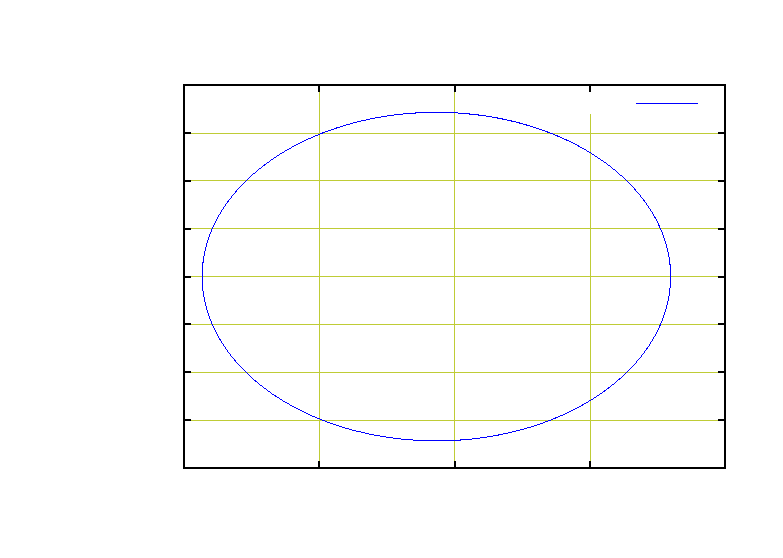
\includegraphics{eg1}}%
    \gplfronttext
  \end{picture}%
\endgroup
}
	\caption{Results of the {\tt oscillator.f95} code plotted on a linear scale. }
	\label{orbitstuff}
\end {figure}

\section{Summary and conclusions}

Hey. HEEEY. Look at fig \ \ref{orbitstuff}. The eigenfunctions $\Psi$ for the first eight energy states were plotted. The graph demonstrates that as $n$ increases the amplitude decreases and the wavelength decreases.

\begin{thebibliography}{}


\bibitem{metcalf} M.\ Metcalf, J.\ Reid and M.\ Cohen, {\it Fortran 95/2003 explained}. Oxford University Press, 2004.
 

\end{thebibliography}




\end{document}
